\section{Evaluation protocol for traceability solutions}\label{sec:evaluation}
\sideboxbegin{o}
This section presents {a protocol to evaluate tracers}. The main focus in the consideration of the trace artefacts themselves, their customization, identification, visualization, persistence and quality assessment. It also sketches {a protocol to integrate Trace\textit{a}'s quality definition into tracers}.
\sideboxend

The quality of traceability solutions lies on five main pillars : 
(1) The customization of the tool to adapt to different systems\footnote{We call \textit{system} or \textit{software system} interchangeably here, considering a software system an abstract representation of a (software) system.}, 
(2) the level of automation of the identification of traces, 
(3) the means of visualisation and retrieval of trace links, 
(4) the means of persistence and additional operations available, 
and (5) level of quality assessment of the tracing constituents.
In this section, we present these as five independent dimensions for the evaluation of traceability solutions. 

\Fig{fig:evaluationpoints} schematizes the overall traceability infrastructure. It shows the three main components: the traces and their constituents, the environment in which it operates, and the artefacts it targets on (a) system (of systems). The figure shows where the dimensions for evaluation apply.
 
\begin{figure}[h]  
	\centering
	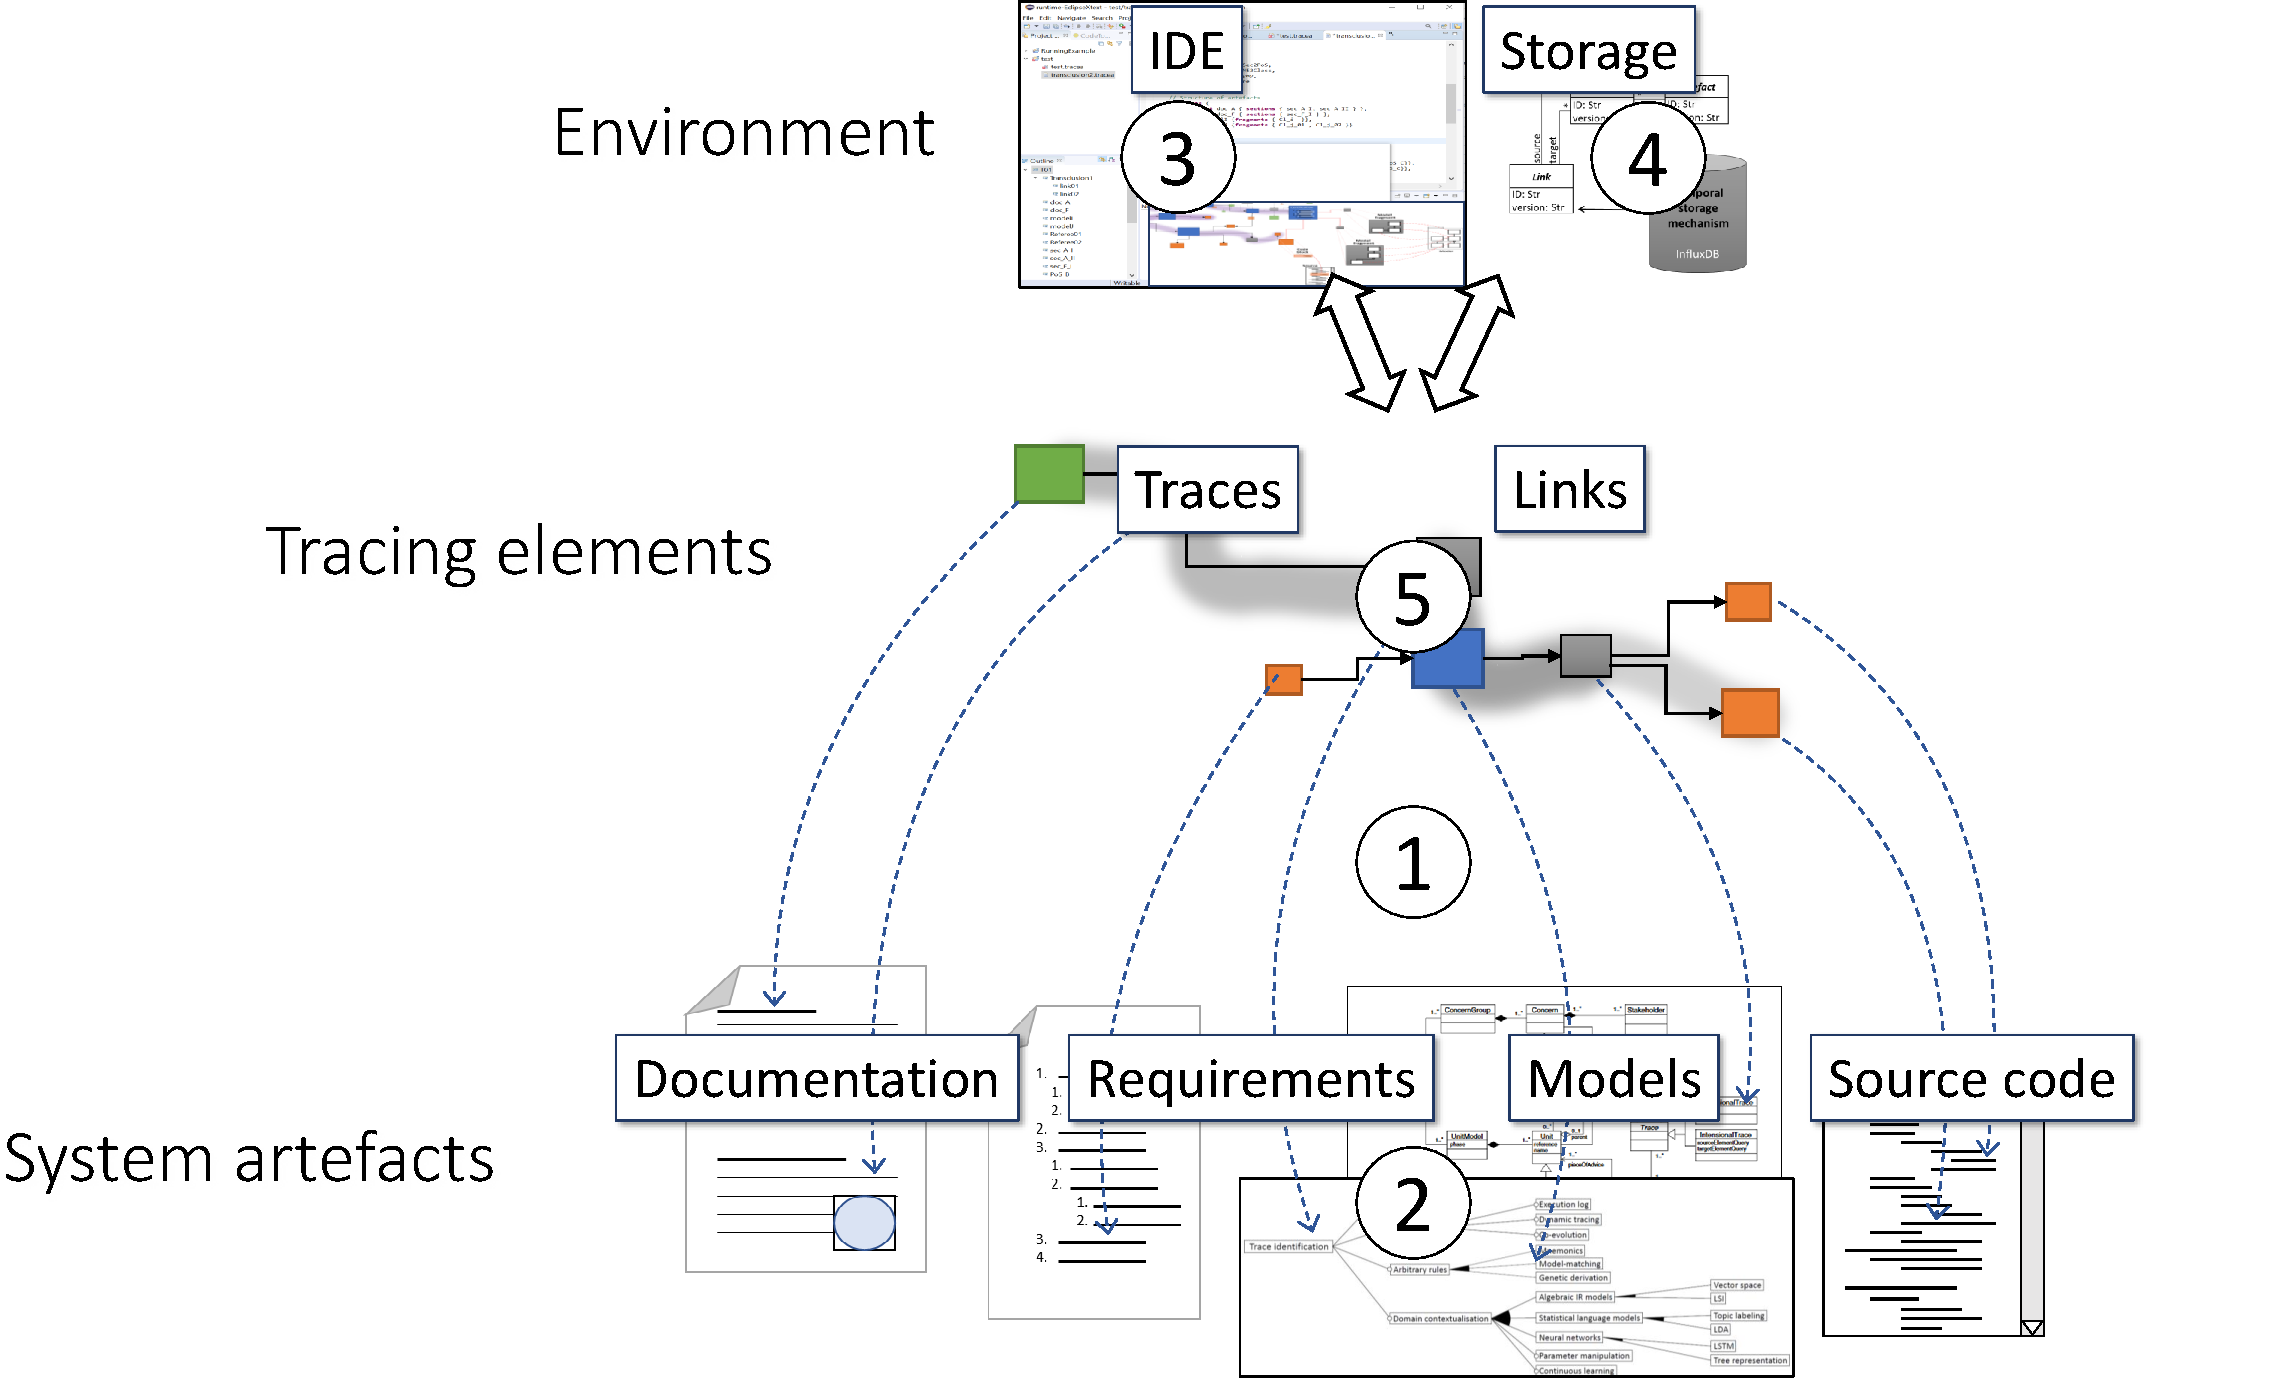
\includegraphics[width=.85\linewidth]{images/evaluation-points.pdf}
	\caption{Overview of the traceability infrastructure with localisation of the dimensions for evaluation}
	\label{fig:evaluationpoints}
\end{figure}

\subsection{Evaluation of traceability solutions}\label{sec:protocol-evaluation}
In more details, we define five dimensions to evaluate a solution to traceability (as summarized in Table \ref{tab:evaluationtable}).
\begin{table}[h]  
	\centering
	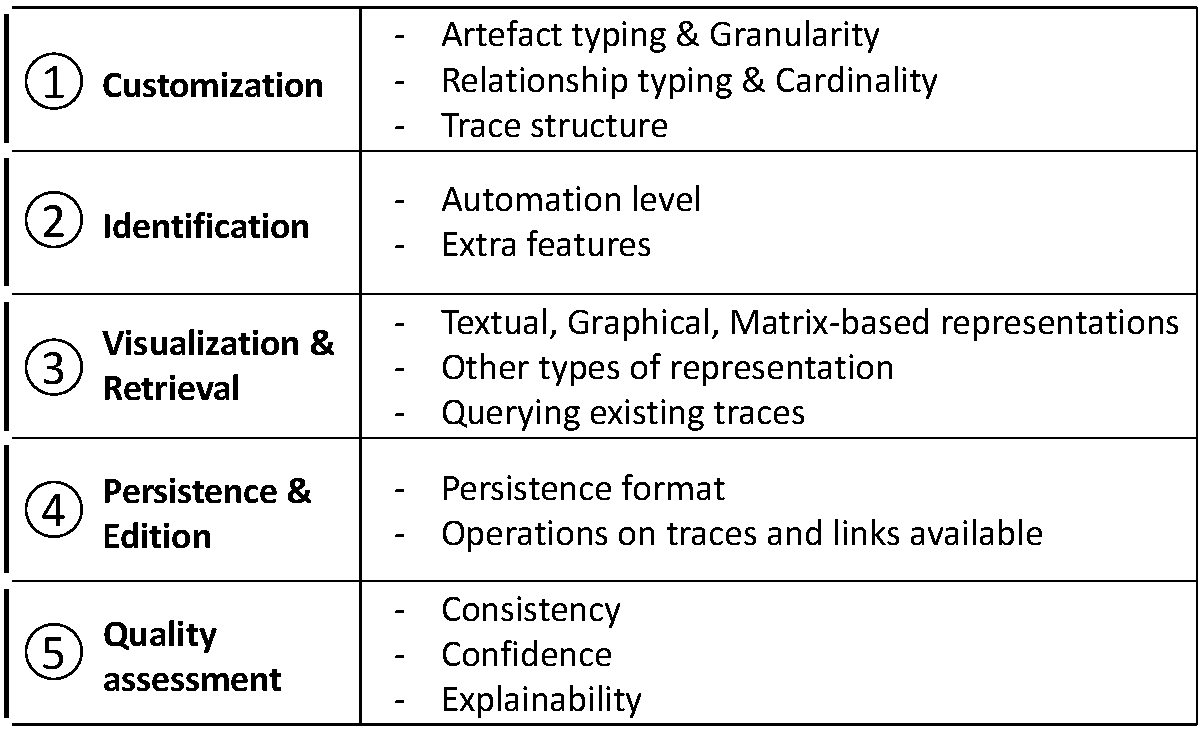
\includegraphics[width=.65\linewidth]{images/evaluation-table.pdf}
	\caption{Five pillars for traceability evaluation.}
	\label{tab:evaluationtable}
\end{table}

\begin{descriptioncompact}
    \item[1 - Customization] To evaluate the potential a tool has to address a specific purpose, \textbf{customizability} must be evaluated with regard to the kind of artefacts and the kind of links it offers to manipulate\footnote{We call "trace links", "connections", "relationships", simply \textit{links} in this document, as opposed to \textit{trace} which are entities composed with (successive) links.}. A generic tooling must allow an \textit{ad hoc} definition of types to adapt to different uses in different application domains \cite{maro2016_maintenance_factors_and_guidelines}. 
    
    \item[2 - Identification] What are the means available for the identification of trace links? This task can be automated to different levels. Links can be identified manually, which usually depends on the integration of the tool into the system's environment. Links can also be identified automatically using rules and/or AI techniques.
    Moreover, there exists explicit links in the syntax trees of many languages. These can be automatically derived, included or used for visualization purpose as an extra feature (or known neighborhood). 

    \item[3 - Visualization \& Retrieval] Once traces are identified, they can be represented in form that fit the needs of the user. \textit{E.g.}, either textually, or diagramatically, in spreadsheet or even in matrix, revealing their structure in a (more or less) legible way, and editable to a certain degree.  
    Matrix-based representations show a broader aspect of the traces in a more "conventional" way that some favor \cite{li2013-trace-matrix-analyzer}. For example, the matrix view makes it easy to see if all requirements are associated to test cases.
    
    There might as well be a great number of traces identified, for various purposes, and a proper tooling to retrieve traces of interest is important. This can be done, for example, with a query-based mechanism.

    \item[4 - Persistence \& Edition] The format in which traces are serialized matters. It can be embedded in the artefacts themselves, or external to the software through independent traceability artefacts. These can be store as model elements, SQL scripts, or XML sheets, and so on depending on traceability requirements (\textit{\eg,} what is most important: expressiveness, efficiency, or interoperability?).
    
    Traces are complex entities and a robust tooling should also offer robust operations to handle them with precision and efficacy.
    
    \item[5 - Quality assessment] Finally, how is the quality of the trace and its constituent assessed? Traces suffer gradual decay, depending on the degree of versatility of the system, they might not be kept up-to-date, and their consistency with the system's artefacts may decline. This indicates that traces might suffer some uncertainty. Is the confidence about the degree of existence of a trace evaluated? Is it possible to record and reuse it? If a trace has been identified automatically, traces should refer to evidences about the rationale behind their identification. Is the tool offering any means to express these considerations?
\end{descriptioncompact}
 

\subsection{Extension for trace quality}\label{sec:protocol-extension}
We foresee a recurring lack in the fulfilment of the last dimension "5 - Quality assessment". All approaches we have seen so far are oblivious of this aspect~\cite{deliverable2,batot2020-survey-driven-feature-model}. We propose to address this limitation through an extension protocol that integrates trace quality into traceability solutions. \Fig{fig:mm-explainability} shows an excerpt of Trace\textit{a} dedicated to the quality of traces and links. This excerpt features confidence values associated with evidences - when they exist. The root element for tracer must also refine \texttt{TracingElement} to advocate for \texttt{Agent} responsibility in the tracing process. A detailed review of {the conceptual modeling beyond trace quality classes} imported by Trace\textit{a} is provided in \cite{batot2021-not-another-metamodel}.

\begin{figure}[h]     
	\centering
	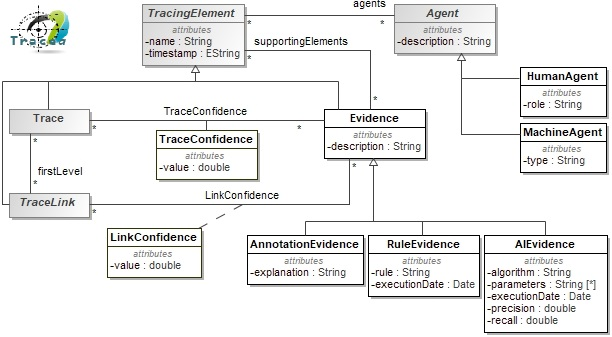
\includegraphics[width=.99\linewidth]{images/mm-explainability.jpg}
	\caption{Excerpt of Trace\textit{a} dedicated to the quality of traces and links.}
	\label{fig:mm-explainability}
\end{figure}


\begin{descriptioncompact}
    \item[1 - Localisation] First of all, we need to locate the core conceptual representation of trace link. Is it a model that generates some low level code? Is it rendered directly in low level code such as Java or C? Is it explicitly modularised or is it part of a bigger picture?
    
    
    The extension point for tracers to integrate Trace\textit{a} lies in the left-hand classes \texttt{Trace} and \texttt{TraceLink} of Fig. \ref{fig:mm-explainability}. Both are susceptible to give a confidence value, supported by evidences if any. 
    %The actual representation of traces and links must be studied as well. Are \textit{traces} actual entities? Or are they \textit{derived} from \textit{links}? 
    
    
    \item[2 - Injection] Then, Trace\textit{a} quality properties must be added to the definition. This may be done through a modification of the metamodel (in the case of low code generation) or a direct edition of low level code related to links and traces. In both cases, Trace\textit{a} must endorse a translation into the language/technology of the targeted tracer.
    
    
    
    \item[3 - Interfacing] Once quality properties have been added to the tracer, it must be propagated through the different packages/modules of the tool. This implies understanding the general architecture of the tracer to be able to add quality properties as a core feature without \textit{breaking stuff}\footnote{Facebook's mantra for developers has long been "Move Fast and Break Things." After decade long polemic over its legal implication, the Menlo Park company has stepped down. Facebook is now embracing the motto "Move Fast With Stable Infra." }.
    
    \item[4 - Change impact] Finally, a change impact analysis must be operated to ensure the changes do not impact unexpected elements of the tracer. This must be done at the specification, design, source code, and test level.
\end{descriptioncompact}



